%% 
%% Copyright 2019-2024 Elsevier Ltd
%% 
%% This file is part of the 'CAS Bundle'.
%% --------------------------------------
%% 
%% It may be distributed under the conditions of the LaTeX Project Public
%% License, either version 1.3c of this license or (at your option) any
%% later version.  The latest version of this license is in
%%    http://www.latex-project.org/lppl.txt
%% and version 1.3c or later is part of all distributions of LaTeX
%% version 1999/12/01 or later.
%% 
%% The list of all files belonging to the 'CAS Bundle' is
%% given in the file `manifest.txt'.
%% 
%% Template article for cas-dc documentclass for 
%% double column output.

\documentclass[a4paper,fleqn]{cas-sc}

\renewcommand{\abstractname}{} 


\usepackage{subcaption}

\usepackage{multicol}

\usepackage[thinc]{esdiff} % for derivatives

% commands I use a lot
\usepackage{xspace}
\newcommand\thedata {$\{(t_i,h_{\text{obs}, i})\}_{i=1}^{N}$\xspace}
\newcommand\thedatanomath {\{(t_i,h_{\text{obs}, i})\}_{i=1}^{N}}
\newcommand\themodel {$h(t; h_0, \boldsymbol \alpha, \boldsymbol\theta)$\xspace}
\newcommand\themodelnomath {h(t; h_0, \boldsymbol \alpha, \boldsymbol\theta)}
\newcommand\thevars{h_0, \boldsymbol \alpha, \boldsymbol \theta, \sigma^2}

\usepackage{wrapfig}
% If the frontmatter runs over more than one page
% use the longmktitle option.

%\documentclass[a4paper,fleqn,longmktitle]{cas-dc}

%\usepackage[numbers]{natbib}
%\usepackage[authoryear]{natbib}
\usepackage[authoryear,longnamesfirst]{natbib}

%%%Author macros
\def\tsc#1{\csdef{#1}{\textsc{\lowercase{#1}}\xspace}}
\tsc{WGM}
\tsc{QE}
%%%

% Uncomment and use as if needed
%\newtheorem{theorem}{Theorem}
%\newtheorem{lemma}[theorem]{Lemma}
%\newdefinition{rmk}{Remark}
%\newproof{pf}{Proof}
%\newproof{pot}{Proof of Theorem \ref{thm}}

\begin{document}
\let\WriteBookmarks\relax
\def\floatpagepagefraction{1}
\def\textpagefraction{.001}

\renewcommand{\thepage}{S\arabic{page}}  
\renewcommand{\thesection}{S\arabic{section}}   
\renewcommand{\thetable}{S\arabic{table}}   
\renewcommand{\thefigure}{S\arabic{figure}}
\renewcommand{\theequation}{S\arabic{equation}}

% Short title
\shorttitle{}    

% Short author
\shortauthors{}  

% Main title of the paper
\title [mode = title]{
Supporting Information: Scanning the cross-sectional area of a solid inside an opaque tank 
  via liquid level dynamics during draining
 }  

% Title footnote mark
% eg: \tnotemark[1]
\tnotemark[1] 

% Title footnote 1.
% eg: \tnotetext[1]{Title footnote text}
\tnotetext[1]{} 

% First author
%
% Options: Use if required
% eg: \author[1,3]{Author Name}[type=editor,
%       style=chinese,
%       auid=000,
%       bioid=1,
%       prefix=Sir,
%       orcid=0000-0000-0000-0000,
%       facebook=<facebook id>,
%       twitter=<twitter id>,
%       linkedin=<linkedin id>,
%       gplus=<gplus id>]

\author[1]{Gbenga Fabusola}%[<options>]

% Credit authorship
% eg: \credit{Conceptualization of this study, Methodology, Software}
\credit{}

% Address/affiliation
\affiliation[1]{organization={Oregon State University},
            % addressline={}, 
            city={Corvallis},
%          citysep={}, % Uncomment if no comma needed between city and postcode
            postcode={97331}, 
            state={Oregon},
            country={USA}}

\author[1]{Cory Simon}

% Footnote of the second author
\cormark[1]

% Email id of the second author


% URL of the second author
\ead[url]{}

% Credit authorship
\credit{}


% Corresponding author text
\cortext[2]{Corresponding author}

% Footnote text
\fntext[1]{}


\renewcommand{\abstract}{} % Extremely risky!
\begin{abstract}
\end{abstract}
% For a title note without a number/mark
%\nonumnote{}
% Keywords
\maketitle

\newpage 

\section{Geometry of the tank}
\begin{figure}[h!]
	\centering
	 \begin{subfigure}[b]{0.35\textwidth}
		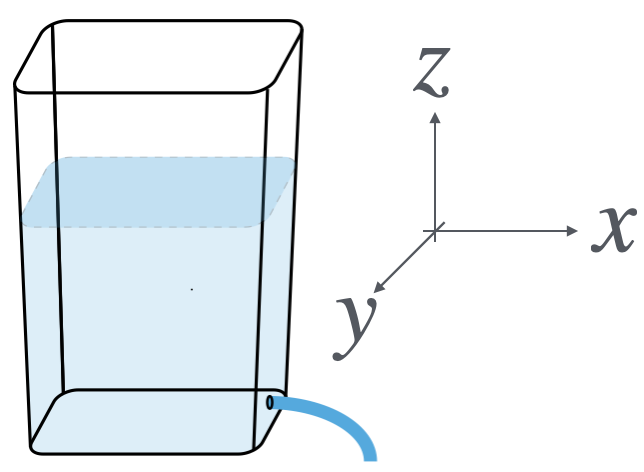
\includegraphics[width=\textwidth]{../drawings_and_photos/views.png} \caption{views of tank}
	\end{subfigure}
	
	\begin{subfigure}[b]{0.8\textwidth}
		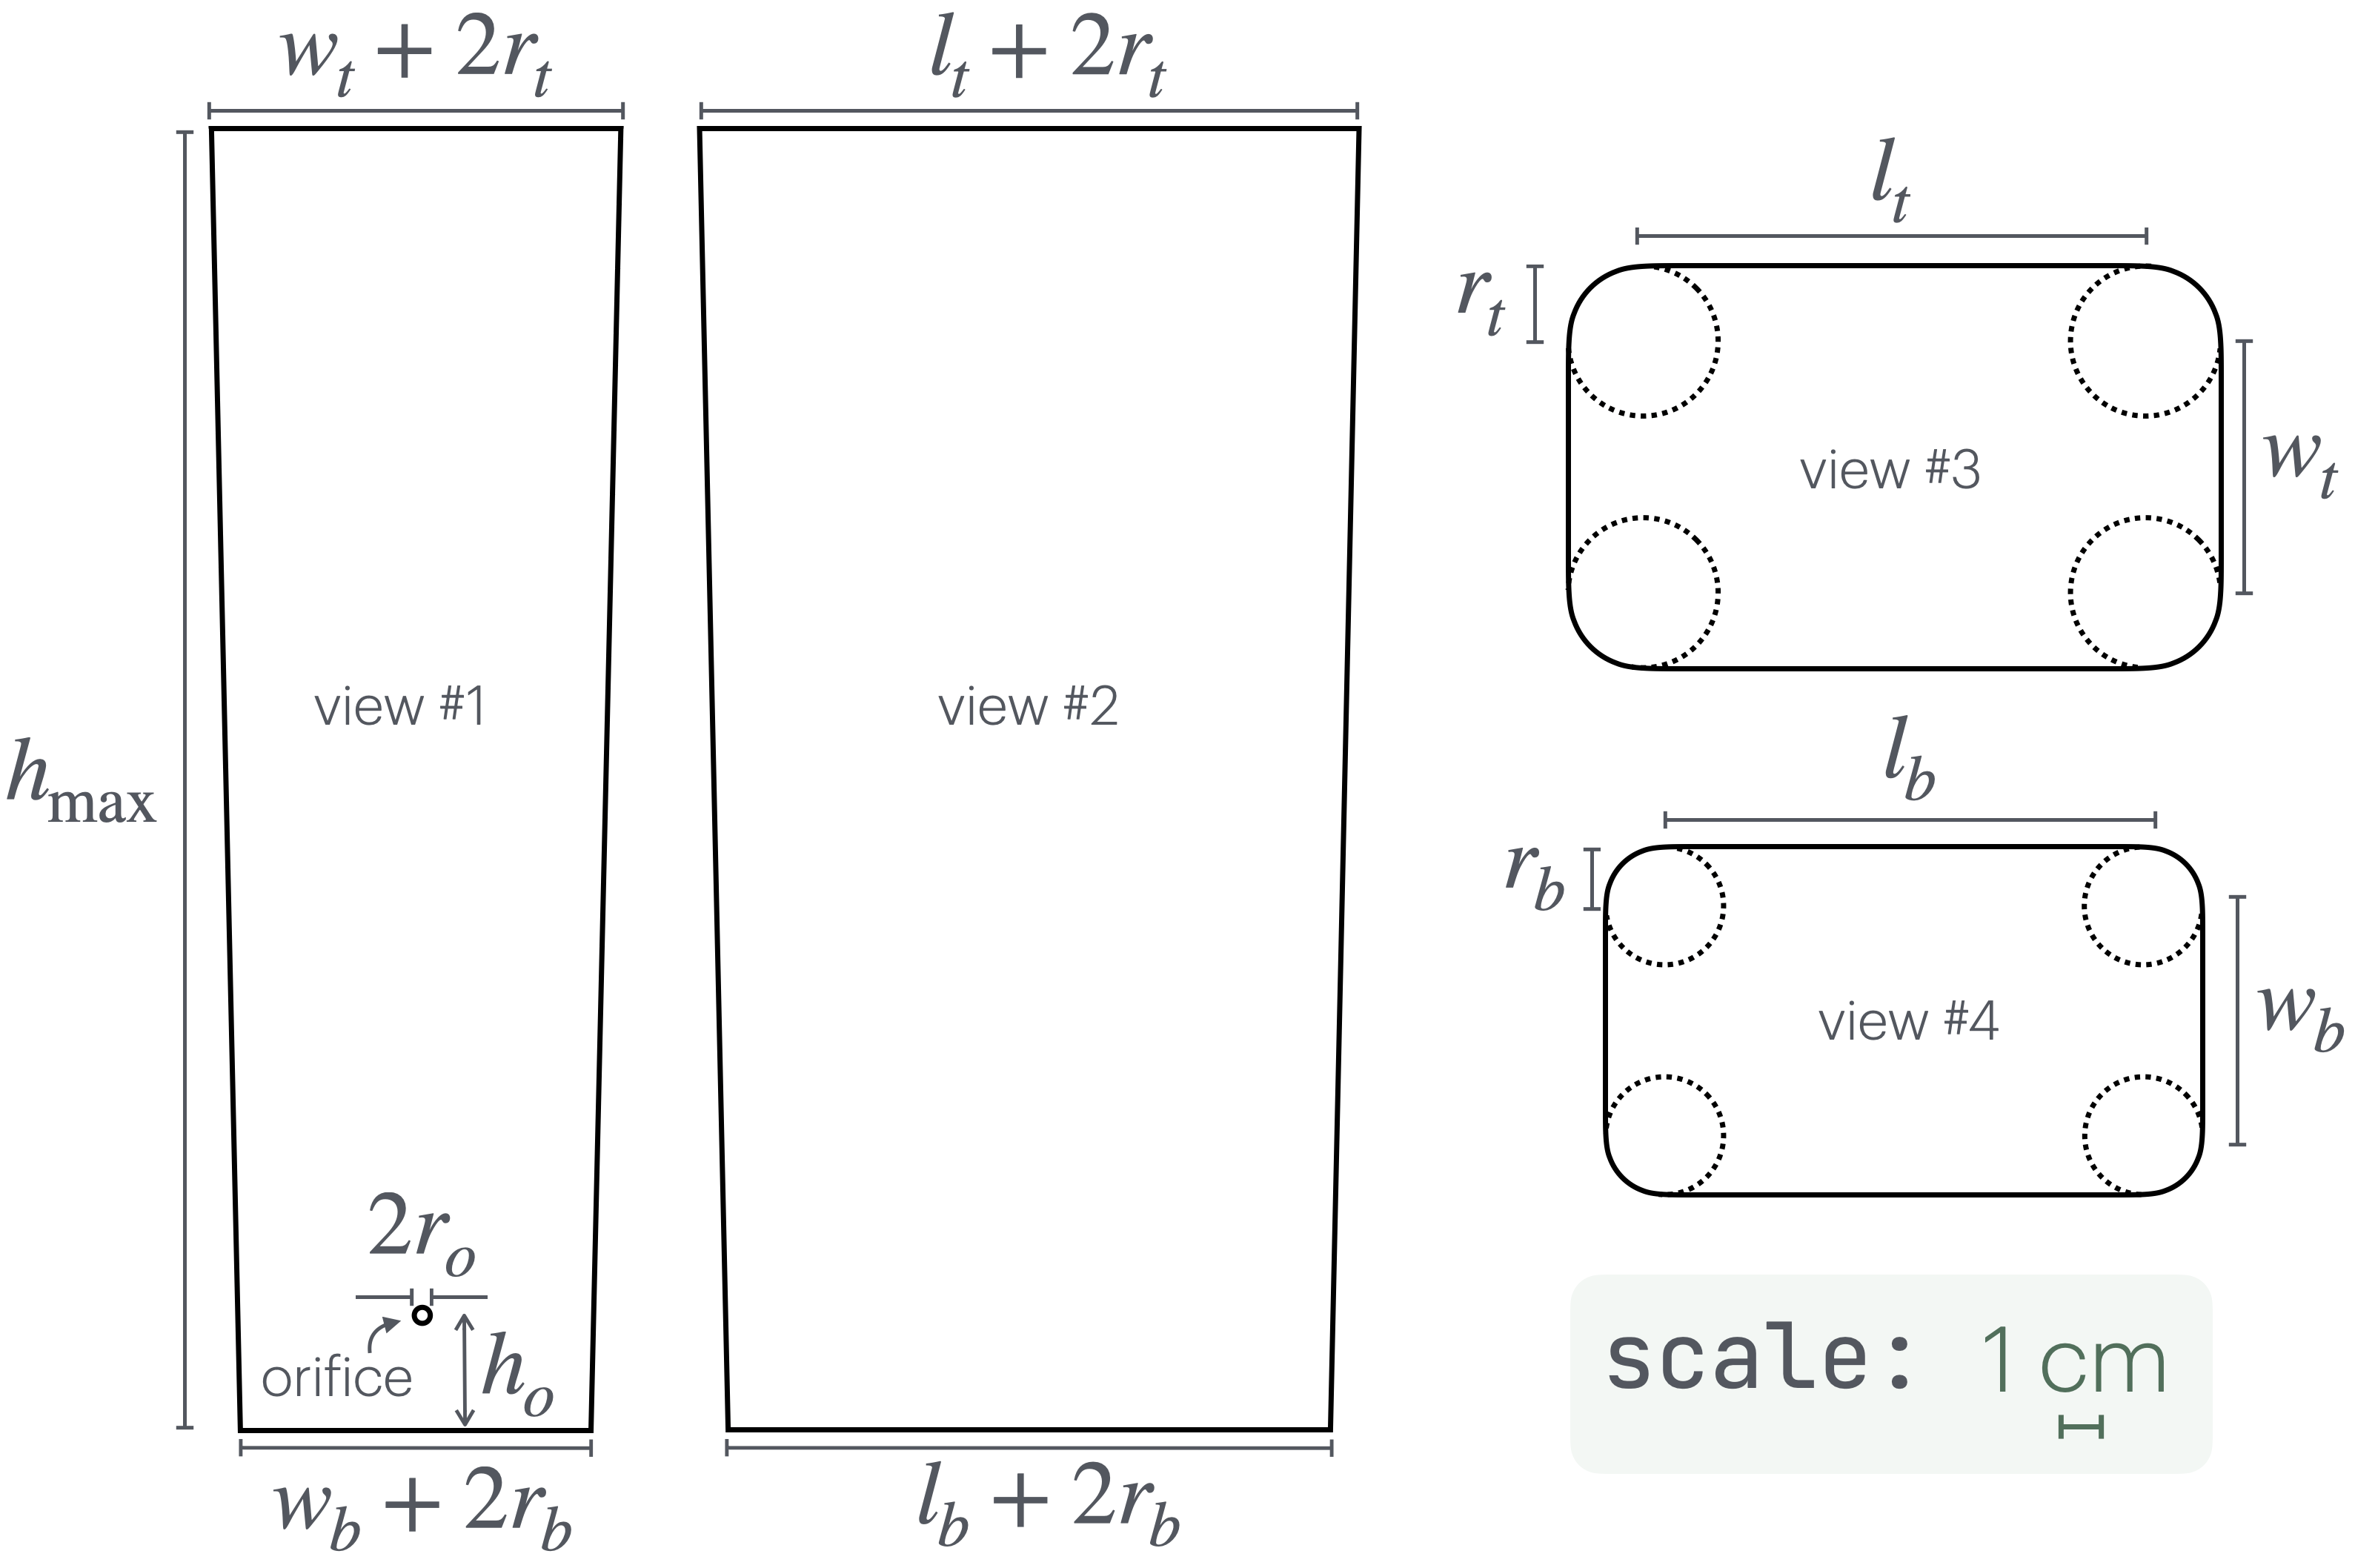
\includegraphics[width=\textwidth]{../drawings_and_photos/tank_geometry.png} \caption{tank geometry from each view}
	\end{subfigure}
	\caption{Geometry of our tank. 
	(a) The 3D geometry of the tank with the four corresponding views we show. (b) The tank from four views, drawn approximately to scale, with variables denoting the dimensions marked. Each cross-section of the tank, taken parallel with the ground, is a rounded rectangle.
	} \label{fig:tank_geometry}
\end{figure}

\clearpage

\section{A rounded rectangle}
We can most directly measure, with a length measuring tape, the two dimensions $l+2r$ and $w+2r$ across the rounded rectangle and its perimeter 
\begin{equation}
p = 2 l + 2 w + 2 \pi r.
\end{equation}
From these, three measurements, we can determine $l$, $w$, and $r$ via solving the system of three equations.

\begin{figure}[h!]
	\centering
	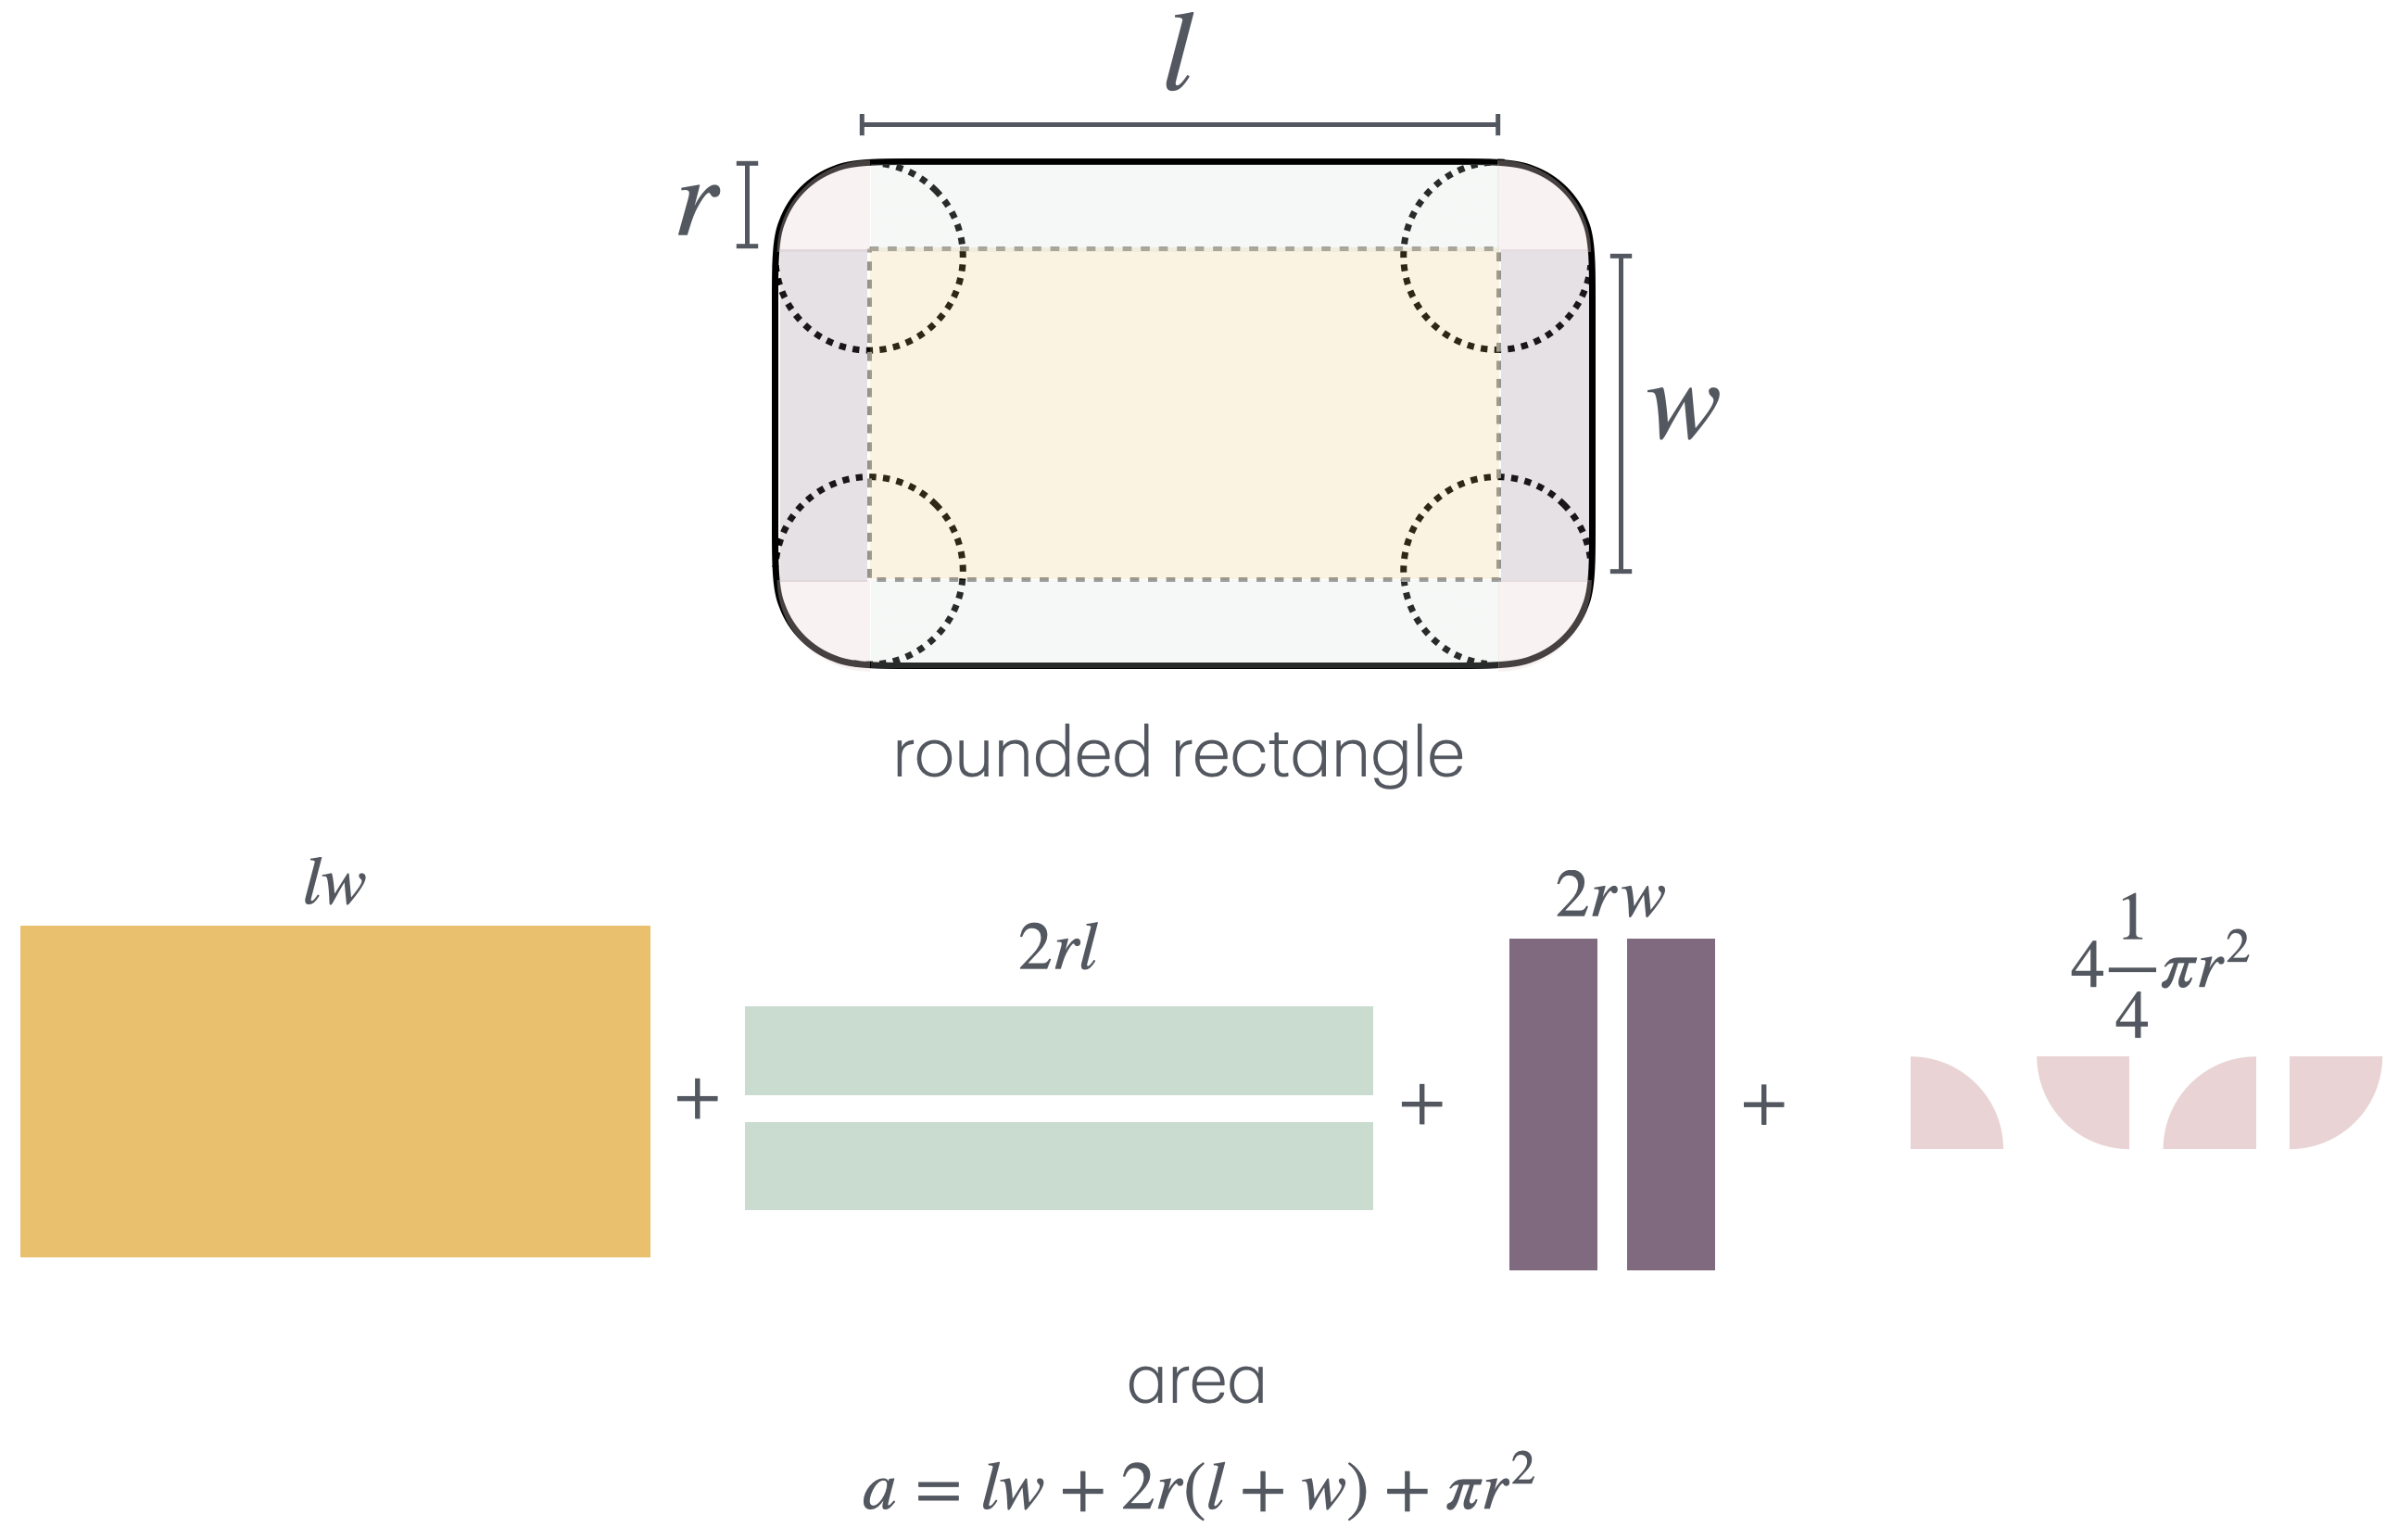
\includegraphics[width=0.75\textwidth]{../drawings_and_photos/rounded_rectangle.png} 
	\caption{A rounded rectangle \cite{rounded_rect} is formed by the convex hull of four circles, each of radius $r$, centered at the four vertices of a rectangle of width $w$ and length $l$. We partition the rounded rectangle into five rectangles and four quarter-circles to visually prove the formula for its area.} \label{fig:rounded_rectangle}
\end{figure}

\clearpage

\section{Cross-sectional area of the tank and solid contained in the tank as a function of height}

\begin{figure}[h!]
	\centering
	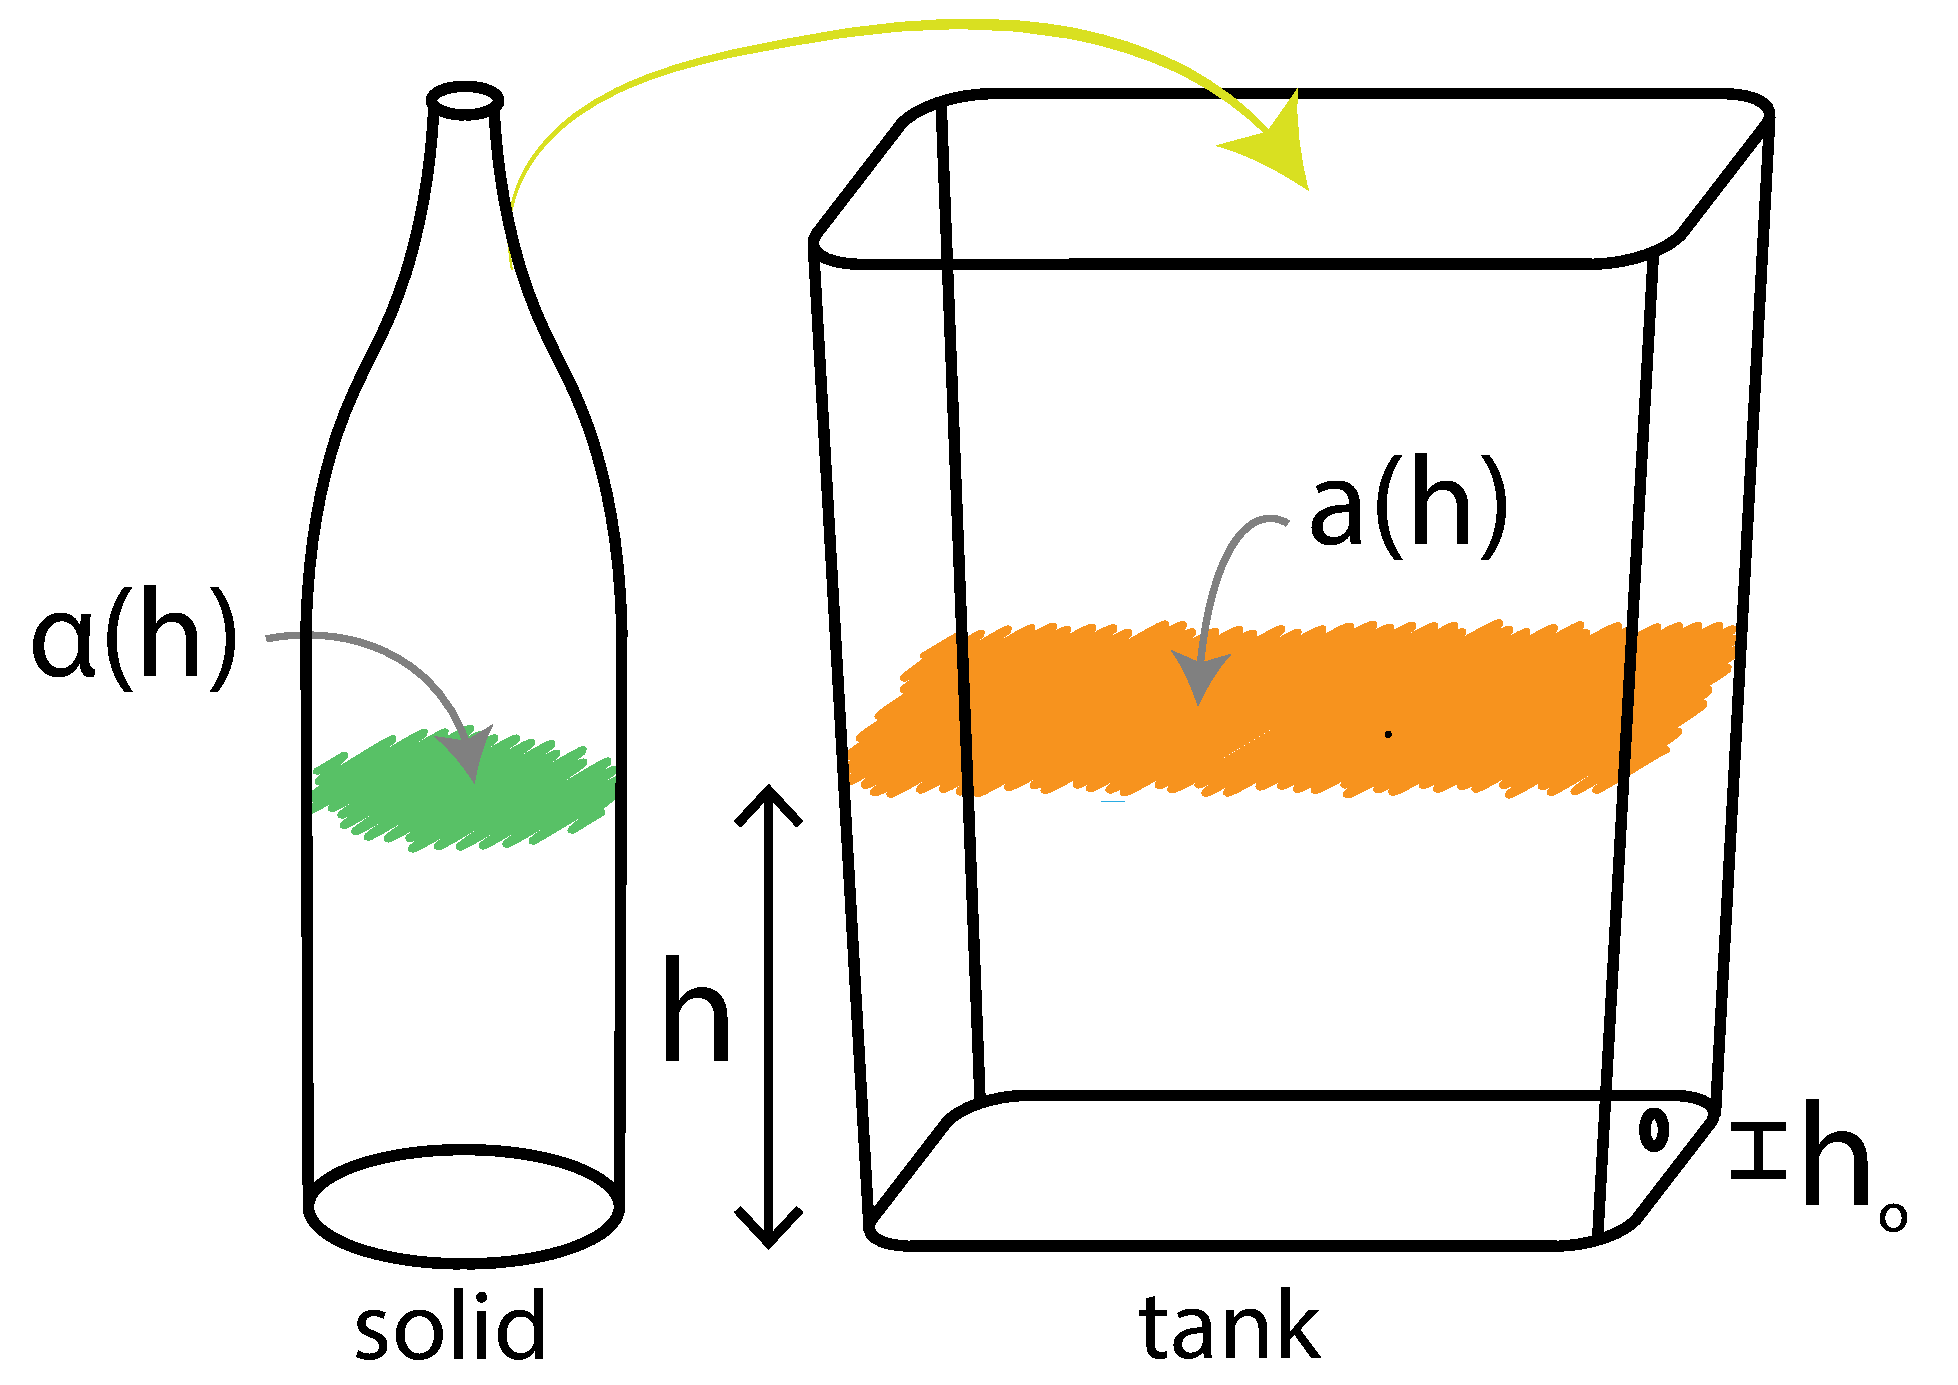
\includegraphics[width=0.75\textwidth]{../drawings_and_photos/a_of_h.pdf} 
	\caption{We illustrate the cross-sectional area, from a helicopter-view, $\alpha(h)$ and $a(h)$, of the exogenous solid and the draining tank, respectively, as a function of height from the ground, $h$. These two functions characterizing the geometry of the tank and exogenous object are key determinants of the dynamics of the liquid level in the draining tank when it contains the exogenous object.}
\end{figure}

\clearpage

\section{Obtaining Torricelli's Law from Bernoulli's Equation}
\label{sec:Torricelli}

\begin{wrapfigure}{r}{0.35\textwidth}
	\centering
	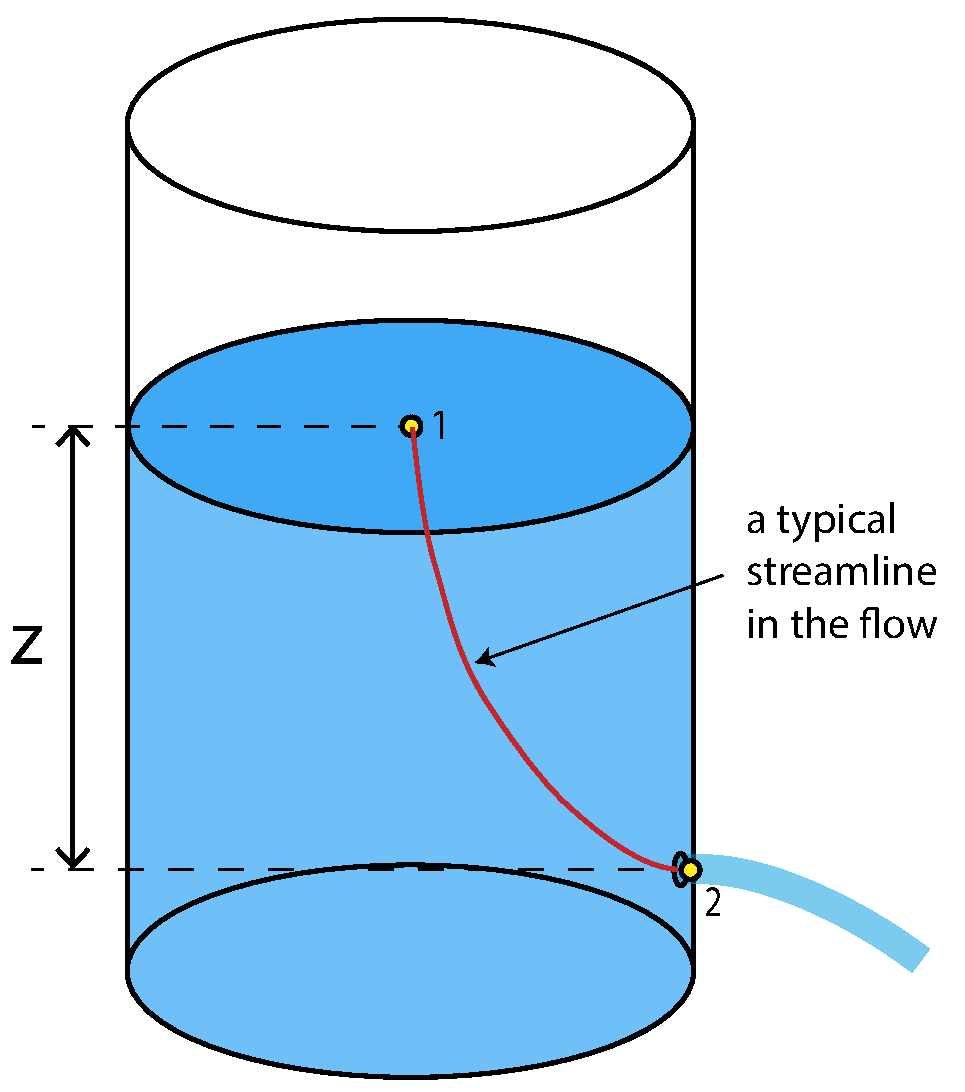
\includegraphics[width=0.35\textwidth]{../drawings_and_photos/torricelli_illustration.pdf}
	\caption{Applying Bernoulli's equation to points (1) and (2) along the typical flow streamline shown gives Torricelli's law after neglecting the small downward velocity of the liquid level in the tank. Sketch mimics Problem 3B.14 in Edition 2 of Bird, Stewart, and Lightfoot \cite{bsl_book}.}
\end{wrapfigure}

	Consider an open-top tank with a small hole in its side. Suppose we nearly fill the tank with liquid then allow liquid to flow out of the tank through the small hole, to the atmosphere. The flow here is driven by the force of gravity.
	At some moment in time, let $z$ [m] be the height of the liquid above the center of the hole. 
	We wish to find the corresponding velocity $v_2$ [m/s] at which the liquid is ejecting from the side of the tank. 
	
	To do so, we follow Bird, Stewart, and Lightfoot \cite{bsl_book} (Problem 3B.14 in Edition 2) by applying Bernoulli's equation to two points in the liquid: 
	(1) a point just below the surface of the liquid at the top of the tank, near the center of the tank, and 
	(2) a point inside the outlet stream, just outside of the tank and near the center of the cross-section of the stream. 
	 Conceptually, we're considering a typical streamline of the flow extending from point (1) to point (2).
	We make three approximations about the liquid along this streamline: 
	(1) the flow is at steady-state (a quasi-steady-state assumption that $z$ is approximately constant at any given instant, justified by it dropping slowly given the large girth of the tank compared to the orifice),
	(2) the liquid is inviscid (i.e., we neglect frictional forces internal to the liquid),
	and
	(3) the liquid is incompressible (i.e., its density, $\rho$ [kg/m$^3$], is constant).
	Also, the flow is isothermal (for our tank draining experiments, we let the water reach room temperature).
	
	A mechanical energy balance then implies Bernoulli's equation \cite{welty2020fundamentals} holds for points (1) and (2) along the flow streamline, which relates the velocity $v_i$ [m/s], pressure $P_i$ [N/m$^2$ $[=]$ kg /(s$^2\cdot$m)], and elevation $y_i$ [m] of the liquid at the two points $i\in\{1,2\}$:
	\begin{equation}
	g y_1 + \frac{1}{2} v_1^2 + \frac{P_1}{\rho} = gy_2 + \frac{1}{2} v_2^2 + \frac{P_2}{\rho} 
	\end{equation}
	where $g$ [m/s$^2$] is the gravitational acceleration constant. 
	
	Now, since both the top of the tank and the stream ejecting from the side of the tank are open to the atmosphere, we have $P_1=P_2=P_a$ with $P_a$ the atmospheric pressure. And, we have $y_1-y_2=z$. Further, we approximate $v_1\approx 0$ since the cross-sectional area of the liquid at the top of the tank is large relative to the cross-sectional area of the hole in the side of the tank (making $v_2 >> v_1$). Bernoulli's equation then reduces to:
	\begin{equation}
	g z  = \frac{1}{2} v_2^2,
	\end{equation}
	which states that the decrease in gravitational potential energy of a parcel of liquid that has traveled from point (1) to (2) matches its gain in kinetic energy from point (1) to point (2). Solving for $v_2$ gives Torricelli's law \cite{driver1998torricelli}:
	\begin{equation}
	v_2 = \sqrt{2gz}.
	\end{equation}
	Torricelli's law states that the velocity of the liquid ejecting from the side of the tank is proportional to the square root of the height of liquid $z$ above the hole, with proportionality constant $\sqrt{2g}$. The gravitational acceleration constant $g$ appears because gravity is the force that drives the flow.
	
\clearpage
	
\section{
A classical method 
to infer 
(a, unknown) the cross-sectional area, as a function of height, of an exogenous solid contained in a tank from 
(b, known) the liquid level dynamics as the tank, of known geometry, drains through a small orifice
}
For comparison to using Bayesian statistical inversion for this inverse problem of reconstruction, we employ a classical (i.e., non-Bayesian nor probabilistic) method here.

 \subsection{Forward model} Still, our forward model
\begin{align}
& \left[ a(h)-\alpha(h)\right] \diff{h}{t}= -c \pi r_o^2 \sqrt{2g (h(t)-h_o)}, \,\,\, t \geq 0\label{eq:SI_model} \\
& h(0)=h_0, \nonumber 
\end{align}
 governs the liquid height $h(t)$ in our draining tank over time $t \geq 0$.
 The cross-sectional area of the tank as a function of height $h$, $a(h)$, is known and characterized by our length measurements.
 
 \subsection{Parameter identification}
 To identify the discharge coefficient $c$, we use the experimental time series data of the liquid level $\{(t_i, h_i)\}_{i=0}^N$ from the tank drainage experiment where the tank does \emph{not} contain an exogenous object, so $\alpha(h) = 0$ $\forall h$. We then define a least-squares loss function:
 \begin{equation}
 	\ell(c) = \displaystyle\sum_{i=1}^N [h_i - h(t_i; c)]^2
 \end{equation} where $h(t;c)$ is the predicted liquid level (i.e. according to the model) at time $t$ if the discharge coefficient were $c$, given by eqn.~\ref{eq:SI_model} under $\alpha(h)=0$, the measured initial liquid level $h_0$, and measured orifice radius and height $r_o$ and $h_o$. (We use $g=9.8$ m/s$^2$.)
 Using a numerical routine (Brent's method \cite{brent2013algorithms}, which does not require a derivative) to minimize $\ell(c)$, we find the discharge coefficient of best-fit is $c^*=0.68$. Fig.~\ref{fig:mle} compares the model $h(t;c^*)$ with the optimal $c^*$ and the time series data $\{(t_i, h_i)\}_{i=0}^N$ used for the fitting.
 
 \subsection{Reconstruction}
Now that we have identified the discharge coefficient $c=c^*$, we use the forward model in eqn.~\ref{eq:SI_model} to tackle the inverse problem of reconstruction: given new liquid level time series data $\{(\hat{t}_i, \hat{h}_i)\}_{i=0}^{\hat{N}}$ from a tank drainage experiment when the tank \emph{does} contain an exogenous solid, predict the cross-sectional area of the exogenous solid as a function of height, $\alpha(h)$. For this task, we solve the forward model in eqn.~\ref{eq:SI_model} for the unknown we seek, using the identified value for the discharge coefficient:
\begin{equation}
\alpha(h) = a(h) +  \frac{c^* \pi r_o^2 \sqrt{2g (h-h_o)}}{\diff{h}{t}}. \label{eq:alpha_unknown}
\end{equation} 
Now, to obtain a prediction for $\alpha(h)$, we need a scheme to approximate $\diff{h}{t}$ as a function of $h$ using the time series data $\{(\hat{t}_i, \hat{h}_i)\}_{i=0}^{\hat{N}}$. Then, $\alpha(h)$ follows. (Again, we take $a(h)$ for the tank as known.)

We employ smoothed, quartic splines (implemented in the DIERCKX library \cite{dierckx1995curve}) to estimate $h(t)$ from the time series data $\{(\hat{t}_i, \hat{h}_i)\}_{i=0}^{\hat{N}}$ from the draining experiment with the exogenous solid, from which $\diff{h}{t}$ follows through differentiation.
Fig.~\ref{fig:spline_fit} shows: on the top panel, the data $\{(\hat{t}_i, \hat{h}_i)\}_{i=0}^{\hat{N}}$ along with the smoothed, quartic spline fit to the data giving our approximation of $h(t)$; and, on the bottom panel, the approximated time-derivative of the liquid level $\diff{h}{t}$ as a function of time, according to the spline representation of $h(t)$. At each point in time, Fig.~\ref{fig:spline_fit} gives a pair $\left(\diff{h(t)}{t}, h(t)\right)$ for the approximation of $\alpha(h)$ at some $h$ via eqn.\ref{eq:alpha_unknown}.

Finally, a classical solution to the reconstruction problem: Fig.~\ref{fig:classical_soln} visualizes the predicted cross-sectional area of the exogenous object as a function of height, $\alpha(h)$, following from eqn.~\ref{eq:alpha_unknown} when we use the smooth splines visualized in Fig.~\ref{fig:spline_fit} for $h(t)$ and $\diff{h(t)}{t}$. For comparison, we also show the directly-measured (via length-measurements) area of the exogenous object as a function of height. 
We obtain a reasonable prediction of the solid's area as a function of height. 
However, unlike our Bayesian statistical inversion in the main text, the uncertainty in the predicted cross sectional area of the solid is not captured.
(Note, in Fig.~\ref{fig:classical_soln} we visualize the square root of the cross-sectional area of the object $\sqrt{\alpha(h)}$ since this has more perceptible units of length.

\begin{figure}[h!]
	\centering
	\begin{subfigure}[b]{0.48\textwidth}
		\includegraphics[width=\textwidth]{classic_MLE_fit.pdf} \caption{} \label{fig:mle}
	\end{subfigure}
	
	 \begin{subfigure}[b]{0.5\textwidth}
		\includegraphics[width=\textwidth]{classical_spline_fit.pdf} \caption{} \label{fig:spline_fit}
	\end{subfigure}
	\begin{subfigure}[b]{0.4\textwidth}
		\includegraphics[width=\textwidth]{classical_soln.pdf} \caption{} \label{fig:classical_soln}
	\end{subfigure}
	\caption{A classical approach to the inverse problem of reconstruction.
	(a) We use liquid level time series data in the draining tank when it does not contain an exogenous object to identify the discharge coefficient $c$ via minimizing a least-squares loss function. The model with the identified discharge coefficient $c^*$ (fit to the data) is shown.
	(b) (top) Liquid level time series data in the draining tank when it contains an exogenous object, along with a smoothed, quartic spline fit to the data for representing $h(t)$. (bottom) The time-derivative of the liquid level according to the spline representation of $h(t)$ on top.
	(c) The measured and predicted square root of the area of the exogenous object as a function of $h$.
	}
\end{figure}

\clearpage

\section{Expanded derivation of the forward model from a mass balance}


% Biography
%\bio{}
% Here goes the biography details.
%\endbio

%\bio{pic1}
% Here goes the biography details.
%\endbio

\clearpage

\bibliographystyle{elsarticle-num}

% Loading bibliography database
 \bibliography{refs}

\end{document}

